%
% IMPORTANT: THIS TEMPLATE NEEDS TO BE COMPILED WITH XeLaTeX
%
% This template uses several fonts not included with Windows/Linux by
% default. If you get compilation errors saying a font is missing, find the line
% on which the font is used and either change it to a font included with your
% operating system or comment the line out to use the default font.
% 


\documentclass[letterpaper, article]{deedy-resume-openfont}


\begin{document}

%%%%%%%%%%%%%%%%%%%%%%%%%%%%%%%%%%%%%%
%
%     TITLE NAME
%
%%%%%%%%%%%%%%%%%%%%%%%%%%%%%%%%%%%%%%


\namesection{Aaron}{Wubshet}
{awubshet@mit.edu | 404.563.9110}

%%%%%%%%%%%%%%%%%%%%%%%%%%%%%%%%%%%%%%
%
%     COLUMN ONE
%
%%%%%%%%%%%%%%%%%%%%%%%%%%%%%%%%%%%%%%
\hfill

\begin{minipage}[t]{0.66\textwidth} 
%%%%%%%%%%%%%%%%%%%%%%%%%%%%%%%%%%%%%%
%     EXPERIENCE
%%%%%%%%%%%%%%%%%%%%%%%%%%%%%%%%%%%%%%
\vspace{.01cm}
\section{Experience}

\runsubsection{Draper}
\descript{| Signal Engineering Intern }
\location{Jan \& June - Aug 2017 | Cambridge, MA}
\vspace{\topsep} % Hacky fix for awkward extra vertical space
\begin{tightemize}
	\item Used a universal software radio peripheral (USRP) and laptop set up using GNU Radio to create local GSM network. 
	\item Created a sector level LTE simulator implemented using MatLab to model aggregate power levels with variable input channel propagation models 
\end{tightemize}
\sectionsep

\runsubsection{Bain \& Company}
\descript{| Building Entreprenuerial Leaders Program Particpant}
\location{Aug 2017| Atlanta, GA}
\begin{tightemize}
	\item Introduced to strategic consulting and accelerated learning opportunities for prospective consultants
	\item Worked alongside Bain case team to tackle real Bain client's business issue
\end{tightemize}
\sectionsep

\runsubsection{MIT Consulting Group}
\descript{| Treasurer and Technical Consultant }
\location{Feb 2016 – Present | Cambridge, MA}
\begin{tightemize}
	\item Manage a quarterly budget of approximately \$ 20,000 as treasurer while providing clients with a wide array of consulting services including prototype testing, market penetration strategies, employee retention plans, wage matrix evaluation, geographic market analysis, and partnership evaluation. 
	\item Clients range from big tech to start-ups to cash-in-transit
\end{tightemize}
\sectionsep

%\runsubsection{MIT Teaching Faculty}
%\descript{| Electrical Engineering and Physics }
%\location{Feb 2016 – Present | Cambridge, MA}
%\begin{tightemize}
%	\item Taught Electricity and Magnetism under Prof. Dourmashkin for 8.02 using the Technology Enabled Active Learning (TEAL) format 
%	\item Served as a lab assistant for Theory and Application of Circuits and Electronics on under Prof. Berggren for 6.169
%\end{tightemize}
%\sectionsep

\runsubsection{MIT MakerLodge}
\descript{| Electronics Team Lead and WebMaster}
\location{Feb 2017 – Present | Cambridge, MA}
\begin{tightemize}
	\item MIT MakerLodge is an initiative to create a centralized shop training infrastructure for undergraduates to learn how to use shop tools ranging from laser cutters to drill presses to soldering irons. 
	\item Served as the co-head of the electronics training team guiding students through basic a training involving soldering, circuit design, and debugging as well as WebMaster to keep trainings sign up slots accessible to freshmen
\end{tightemize}

%%%%%%%%%%%%%%%%%%%%%%%%%%%%%%%%%%%%%%%
%%     Projects
%%%%%%%%%%%%%%%%%%%%%%%%%%%%%%%%%%%%%%%

\section{Projects}

\runsubsection{Speaker Tracking System}
\\
\location{Apr - May 2017 | Cambridge, MA}
\begin{tightemize}
	\item Created a target following speaker system that turned to face the target as it moved around as well automatically adjusting the volume
	\item Designed and implemented the system using an Intel microcontroller as well as Cypress PSoC Bluetooth module
\end{tightemize}

\runsubsection{Noise Cancellation}
\\
\location{Mar - Apr 2017 | Cambridge, MA}
\begin{tightemize}
	\item Investigated and simulated noise cancellation methods using basic feedback control patterns as well as designed custom physical speaker system enclosure
	\item Built circuitry to recreate the simulation results on the physical speaker 
\end{tightemize}

\runsubsection{Movie Rating WebApp}
\\
\location{September 2016 | Cambridge, MA}
\begin{tightemize}
	\item Created a Firebase powered social multimedia platform with a feedback based value system where group members have a time changed vote weight depending on past reliability in picking enjoyable movies
\end{tightemize}

%\runsubsection{Wireless Charger}
%\\
%\location{Aug 2013 – May 2014 | Lawerenceville, GA}
%\begin{tightemize}
%	\item Designed and built circuitry to wirelessly charge a cell phone from a distance of about one meter as part of an Intel Science Fair project submission
%\end{tightemize}
%\sectionsep

%%%%%%%%%%%%%%%%%%%%%%%%%%%%%%%%%%%%%%
%     RESEARCH
%%%%%%%%%%%%%%%%%%%%%%%%%%%%%%%%%%%%%%

%\section{Research}
%
%\runsubsection{RLE at MIT}
%\descript{| Research Assistant}
%\location{Nov 2015 – May 2016 | Cambridge, MA}
%\begin{tightemize}
%	\item Experimentalist and data analyst under Marin Sojacic creating transparent displays with silver and gold nanoparticles dispersed in a polymer matrix
%	\item Experimented with possible ratios of specific nanoparticles to polymer while accounting for size and identity in order to sharpen resonant scattering\\
%\end{tightemize}
%\sectionsep
%
%\runsubsection{Quantum Chemistry Lab at GT}
%\descript{| Research Assistant}
%\location{Aug 2014 – May 2015 | Atlanta, GA}
%\begin{tightemize}
%	\item Experimental apparatus designer under Ken Brown constructing additional laser modulation systems via direct digital synthesis
%	\item Worked with Ca\textsuperscript{2+} ion trapping to investigate quantum states and computers
%\end{tightemize}


\end{minipage} 
\hfill
%%%%%%%%%%%%%%%%%%%%%%%%%%%%%%%%%%%%%%
%
%     COLUMN TWO
%
%%%%%%%%%%%%%%%%%%%%%%%%%%%%%%%%%%%%%%
\begin{minipage}[t]{0.33\textwidth} 

%%%%%%%%%%%%%%%%%%%%%%%%%%%%%%%%%%%%%%
%     EDUCATION
%%%%%%%%%%%%%%%%%%%%%%%%%%%%%%%%%%%%%%
\vspace{\topsep}
\centering{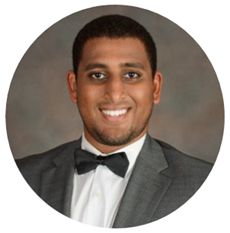
\includegraphics{resume_image.png}}


\section{Education} 

\subsection{Massachusetts Institute of Technology \hfill}
\descript{{\large BS in Electrical Engineering}}
\location{Expected June 2019 | Cambridge, MA \\ GPA: 4.3}
\sectionsep

\subsection{Relevant Coursework \hfill}
\vspace{.05cm}
6.302: Feedback Systems and Controls\\
6.115: Microcomputer Project Laboratory \\



%%%%%%%%%%%%%%%%%%%%%%%%%%%%%%%%%%%%%
%     SKILLS
%%%%%%%%%%%%%%%%%%%%%%%%%%%%%%%%%%%%%%

\section{Skills}
\subsection{Technical}

Inventor/SolidWorkds \hspace{.27cm} \textbullet \textbullet  \textbullet \\
Python \hspace{2.5cm} \textbullet \textbullet \textbullet  \textbullet\\
MatLab \hspace{2.42cm} \textbullet \textbullet \textbullet \textbullet  \textbullet\\ 
Eagle PCB Designer \hspace{.58cm} \textbullet \textbullet \textbullet \textbullet  \textbullet \\
\sectionsep

\subsection{Leadership}
Cash flow and Accounting \hspace{.55cm} \textbullet \textbullet \textbullet  \textbullet\\
Logistics and Organization \hspace{.5cm} \textbullet \textbullet  \textbullet \\
People Management \hspace{1.38cm} \textbullet \textbullet \textbullet \textbullet  \textbullet


\section{Research} 
\subsection{Space Systems Laboratory (SSL) at MIT \hfill}
Designed photodiode amplifier circuit for nanosat electronics team working under Kerri Cahoy 
\sectionsep
\subsection{Research Laboratory of \hfill}
\subsection{Electronics (RLE) at MIT \hfill} 
Experimentalist under Prof. Marin Sojacic creating transparent displays with nanoparticles dispersed in polymer matrix
\sectionsep
\subsection{Cold Molecules and \hfill}
\subsection{Quantum Information \hfill Lab at GT \hfill}
Experimental apparatus designer under Prof. Ken Brown working with laser modulation system to ion trap Ca\textsuperscript{2+}



\end{minipage} 

\end{document}